%%%%%%%%%%%%%%%%%%%%%%%%%%%%%%%%%%%%%%%%%%%%%%%%%%%%%%%%%%%%%%%%%%%%%%
% Problem statement
\begin{statement}[
  problempoints=70,
  timelimit=2 seconds,
  memorylimit=512 MiB,
]{Spiderman}

\setlength\intextsep{-0.1cm}
\begin{wrapfigure}[7]{r}{0.26\textwidth}
\centering
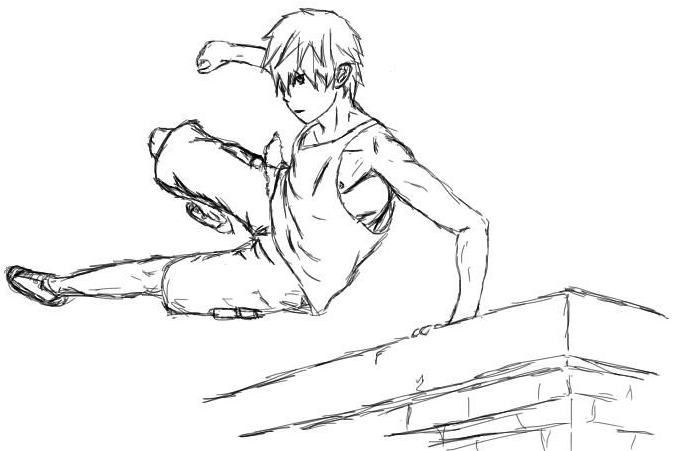
\includegraphics[width=0.26\textwidth]{img/spiderman.png}
\end{wrapfigure}

Little Ivan likes to play \textbf{Yamb} and read Marvel superhero comics.
His favorite superhero is spider-man, a friendly neighbourhood teenager
named Peter Parker who got his superpowers via a radioactive spider bite.
Ivan fantasizes that one day he will be able to jump from one skyscraper to
another, just like spider-man does in the comics. During one such fantasy, he
fell asleep.

In his dream he was no longer named Ivan, his name was Peter Parkour and, you
guessed it, he was able to use his parkour\footnote{Internet sensation of
2004., it was in the Bond films, the goal is to get from point $A$ to point
$B$ as creatively as possible.} skills to jump between skyscrapers. He
quickly realized that there are exactly $N$ skyscrapers in his surroundings
and he somehow knew that $i$-th of those skyscrapers is $h_i$ meters tall. He
knows that he is able to jump from the $i$-th skyscraper to the $j$-th
skyscraper if the remainder when dividing $h_i$ with $h_j$ is equal to $K$.
Help Ivan determine, for every skyscraper, the number of other skyscrapers he
can jump to.

%%%%%%%%%%%%%%%%%%%%%%%%%%%%%%%%%%%%%%%%%%%%%%%%%%%%%%%%%%%%%%%%%%%%%%
% Input
\subsection*{Input}
The first line contains two integers $N$ $(1 \le N \le 300\ 000)$ and $K$
$(0 \le K < 10^6)$ from the task description.

The next line contains $N$ integers $h_i$ $(1 \le h_i \le 10^6)$ from the task
description.

%%%%%%%%%%%%%%%%%%%%%%%%%%%%%%%%%%%%%%%%%%%%%%%%%%%%%%%%%%%%%%%%%%%%%%
% Output
\subsection*{Output}
In a single line you should output $N$ space-separated integers such that the
$i$-th of those integers represents the number of different skyscrapers on
which Peter Parkour can jump on if he jumps from the $i$-th skyscraper.

%%%%%%%%%%%%%%%%%%%%%%%%%%%%%%%%%%%%%%%%%%%%%%%%%%%%%%%%%%%%%%%%%%%%%%
% Scoring
\subsection*{Scoring}
In test cases worth a total of $14$ points, it will hold $1 \le N \le 2\ 000$\\
In test cases worth an additional $14$ points, there will be at most $2\ 000$
skyscrapers of different heights. \\
In test cases worth an additional $14$ points, it will hold $K = 0$.

%%%%%%%%%%%%%%%%%%%%%%%%%%%%%%%%%%%%%%%%%%%%%%%%%%%%%%%%%%%%%%%%%%%%%%
% Examples
\subsection*{Examples}
\begin{tabularx}{\textwidth}{X'X'X}
\sampleinputs{test/spiderman.dummy.in.1}{test/spiderman.dummy.out.1} &
\sampleinputs{test/spiderman.dummy.in.2}{test/spiderman.dummy.out.2} &
\sampleinputs{test/spiderman.dummy.in.3}{test/spiderman.dummy.out.3}
\end{tabularx}

\textbf{Clarification of the third example:}\\
From the first skyscraper of height $1$ Peter can jump on any other skyscraper.\\
From the second skyscraper of height $3$ Peter can jump only on a skyscraper of  height $2$.\\
From the third skyscraper of height $5$ Peter can jump only on a skyscraper of height $2$.\\
From the fourth skyscraper of height $7$ Peter can jump on skyscrapers of heights $2$ and $3$.\\
From the fifth skyscraper of height $2$ Peter cannot jump on any other skyscraper.

%%%%%%%%%%%%%%%%%%%%%%%%%%%%%%%%%%%%%%%%%%%%%%%%%%%%%%%%%%%%%%%%%%%%%%
% We're done
\end{statement}

%%% Local Variables:
%%% mode: latex
%%% mode: flyspell
%%% ispell-local-dictionary: "croatian"
%%% TeX-master: "../hio.tex"
%%% End:
